\section{Centre differencing}
\label{sect:centre}

A more accurate technique using the Taylor expansion method is the centre difference technique. This uses the points either side of the point under examination $t$ (i.e..:\ $t - \Delta t$ and $t + \Delta t$), smoothing the data and producing a more accurate estimate of the numerical derivative at that point. From above, the Taylor series expansion is defined as
\begin{equation}
r(t - \Delta t) = r(t) - r'(t)\Delta t +  \frac{r''(t)}{2!}(\Delta t)^{2} - \frac{r'''(t)}{3!}(\Delta t)^{3}  + ...
\end{equation}
at the point $t - \Delta t$ and 
\begin{equation}
r(t + \Delta t) = r(t) + r'(t)\Delta t +  \frac{r''(t)}{2!}(\Delta t)^{2} + \frac{r'''(t)}{3!}(\Delta t)^{3}  + ...
\end{equation}
at the point $t + \Delta t$. The centre differencing technique subtracts the following point from the leading point:
\begin{equation}
r(t + \Delta t) - r(t - \Delta t)
\end{equation}
This produces the equation
\begin{equation}
r(t + \Delta t) - r(t - \Delta t) = 2 r'(t)\Delta t +  2 \frac{r'''(t)}{3!}(\Delta t)^{3}  + ...
\end{equation}
This equation can then be re-arranged to give
\begin{equation}
r'(t) = \frac{r(t + \Delta t) - r(t - \Delta t)}{2 \Delta t} - \frac{r'''(t)}{3!}(\Delta t)^{2}  + ...
\end{equation}
Following the notation from before, this is usually written
\begin{equation}
r'(t) = \frac{r(t + \Delta t) - r(t - \Delta t)}{2 \Delta t} + O(\Delta t^{2})
\end{equation}
where $O(\Delta t^{2})$ is the truncation error term. The truncation error term in this case is determined by the square of the distance between neighbouring points, producing a more accurate estimate than the forward and reverse difference methods. 

As with the forward and reverse-difference techniques, the velocity estimate produced by the centre-difference method must be multiplied by $10^{3}$ to give the physically realistic units of km~s$^{-1}$, with the acceleration estimate multiplied by $10^{6}$ to give the physically realistic units of m~s$^{-2}$. This has been done for all the simulated data-sets that have been processed using the centre-difference technique.

%\begin{figure}[!t] 
%  \centerline{
%              \includegraphics[width=0.9\textwidth,trim = 0mm 0mm 0mm 0mm,clip=]{images/c_diff_lin.eps}
%              }
%\caption[Centre difference technique simulation]{\emph{Top}: Simulated distance-time data with noise added. \emph{Middle}: Velocity-time data obtained using a centre-difference technique. \emph{Bottom}: Acceleration-time data obtained using a centre-difference technique. }
%\label{fig:c_diff_sim}
%\end{figure}

The centre-difference method effectively smoothes the data set while differentiating it by using the two points either side of the point under examination. The truncation error can once again be given in terms of the original function. From above the truncation error is defined as:
\begin{equation}
O(\Delta t^{2}) = \frac{r'''(t)}{3!}(\Delta t)^{2}
\end{equation}
In this case, the truncation error is defined by the third order derivative of the original function (unlike the second-order derivative for the forward and reverse-difference methods). As before, the third-order derivative can be defined as
\begin{equation}
r'''(t) = \frac{r''(t + \Delta t) - r''(t - \Delta t)}{2 \Delta t} 
\end{equation}
using the definition of the centre-difference technique. Once all of the terms have been re-written in terms of the original equation, the truncation error term, may be written as
\begin{equation}
O(\Delta t^{2}) = \frac{r(t + 3\Delta t) - 3r(t + \Delta t) + 3r(t - \Delta t) - r(t - 3\Delta t)}{(3!)(8)\Delta t}
\end{equation}
This produces a mean truncation error estimate that is much smaller than the mean truncation error calculated using the forward and reverse-difference techniques.

As with the forward and reverse-difference techniques, the truncation error term can be estimated for the acceleration term by using the velocity function $v(t)$ as the base function rather than the distance function $r(t)$. When this is done, it produces the estimate
\begin{equation}
O(\Delta t^{2}) = \frac{v(t + 3\Delta t) - 3v(t + \Delta t) + 3v(t - \Delta t) - v(t - 3\Delta t)}{(3!)(8)\Delta t}
\end{equation}
for the truncation error of the acceleration data. 

The centre-difference technique produces a mean truncation error estimate and a scatter in the data that are much smaller than the forward and reverse-difference techniques. As a result, the centre-difference technique produces a better estimate of the velocity and acceleration, and their associated truncation errors than either the forward or reverse-difference techniques.